\documentclass{article}
\usepackage{tikz}
\usetikzlibrary{arrows.meta, positioning, shapes.multipart}

\begin{document}

\begin{figure}[ht]
\centering
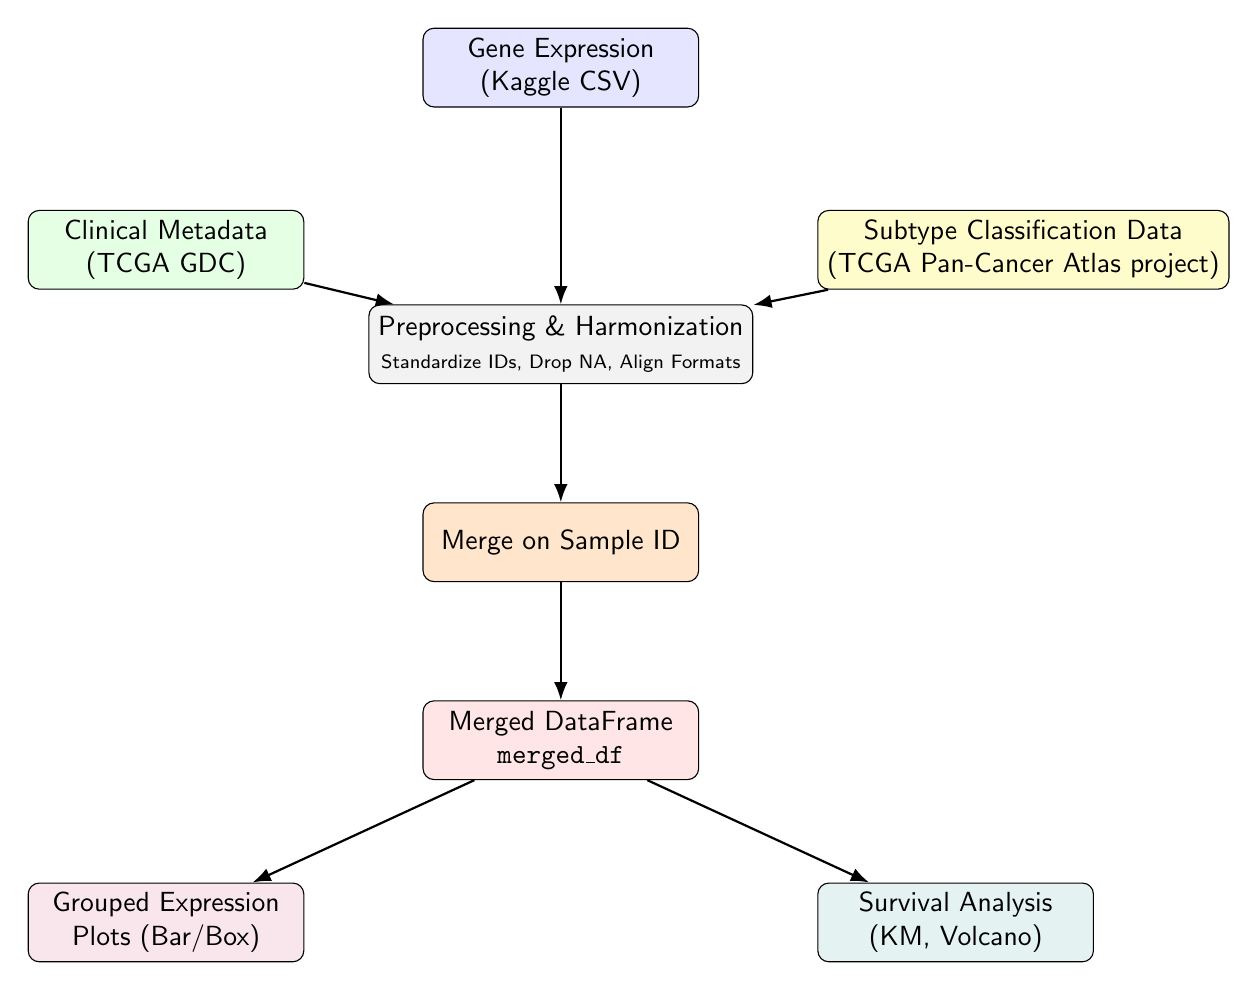
\begin{tikzpicture}[
  node distance=1.3cm and 1.5cm,
  every node/.style={font=\sffamily},
  box/.style={draw, rectangle, rounded corners, align=center, minimum width=3.5cm, minimum height=1cm},
  arrow/.style={-Latex, thick}
]

% Data source nodes
\node[box, fill=blue!10] (expr) {Gene Expression\\(Kaggle CSV)};
\node[box, fill=green!10, below left=of expr] (clinical1) {Clinical Metadata\\(TCGA GDC)};
\node[box, fill=yellow!20, below right=of expr] (clinical2) {Subtype Classification Data\\(TCGA Pan-Cancer Atlas project)};


% Preprocessing
\node[box, fill=gray!10, below=2.5cm of expr] (prep) {Preprocessing \& Harmonization\\\scriptsize Standardize IDs, Drop NA, Align Formats};

% Merge
\node[box, fill=orange!20, below=1.5cm of prep] (merge) {Merge on Sample ID};

% Merged DF
\node[box, fill=red!10, below=1.5cm of merge] (merged) {Merged DataFrame\\\texttt{merged\_df}};

% Output nodes
\node[box, fill=purple!10, below left=of merged] (plot) {Grouped Expression\\Plots (Bar/Box)};
\node[box, fill=teal!10, below right=of merged] (survival) {Survival Analysis\\(KM, Volcano)};

% Arrows
\draw[arrow] (expr) -- (prep);
\draw[arrow] (clinical1) -- (prep);
\draw[arrow] (clinical2) -- (prep);
\draw[arrow] (prep) -- (merge);
\draw[arrow] (merge) -- (merged);
\draw[arrow] (merged) -- (plot);
\draw[arrow] (merged) -- (survival);

\end{tikzpicture}
\caption{Schematic of multi-database integration workflow used in this study.}
\label{fig:multi_db_workflow}
\end{figure}

\end{document}
